%===============================================================================
% $Id: ifacconf.tex 19 2011-10-27 09:32:13Z jpuente $  
% Template for IFAC meeting papers
% Copyright (c) 2007-2008 International Federation of Automatic Control
%===============================================================================
\documentclass[a4paper]{ifacconf}

\usepackage{graphicx,amsmath,url,booktabs}      % include this line if your document contains figures
\usepackage[round]{natbib}             % required for bibliography
\graphicspath{{scripts/figuras/}}
\makeatletter
\def\input@path{{scripts/figuras/}}
\makeatother
\newcommand{\figwidth}{8.8cm}
\newcommand{\figpdforpng}[1]{%
  \IfFileExists{#1.pdf}{\includegraphics[width=\figwidth]{#1.pdf}}{\includegraphics[width=\figwidth]{#1.png}}%
}
%===============================================================================


% ===============================================================
% Choose the language of the manuscript.
% If in English, choose 
% \def\portugues{0} 
%
% If in Portuguese or Spanish, choose
% \def\portugues{1} 
%
% Note that, if you are writing in Spanish, you need additional 
% adjusts in some parts of the text, which have been put in Portuguese only.
\def\portugues{1} 
% ===============================================================

% If the above line is commented, it is assumed manuscript in English:
\ifx\portugues\undefined
\def\portugues{0}
\fi


\if\portugues0
   \usepackage[english]{babel}
  \else
   \usepackage[spanish,brazil,english]{babel}
\fi

  

\usepackage[T1]{fontenc}
%\usepackage{inputenc}

\usepackage[utf8]{inputenc}

\usepackage{ae}


\if\portugues1
% =====================================================================
% =====================================================================
% If the manuscript is in Spanish, please change the texts adequatelly.
% You may also add other definitions in this part.
 \newtheorem{teorema}[thm]{{\em Teorema}}{ }
 \newtheorem{lema}[thm]{{\em Lema}}{ }
 \newtheorem{corolario}[thm]{{\em Corolário}}{ }
 \newenvironment{prova}{{\bf Prova.}}{ }
% ===============================================================
\fi

\begin{document}


\if\portugues1

   % =====================================================================
   % =====================================================================
   % USE THIS PART IF THE TEXT IS IN PORTUGUES OR SPANISH
   % =====================================================================
   % If the manuscript is in Spanish, please change the texts adequately.
   % =====================================================================
   % 
   \selectlanguage{brazil}

   \begin{frontmatter}

      \title{Modelagem e Controle Digital de Pressão por Roda em Módulo Hidráulico de Freio para Frenagem Ativa em ADAS: Estudo em Simulação}
      % Title, preferably not more than 10 words.
      %Modeling and Digital Control of Wheel Brake Pressure in a Hydraulic Brake Module for Active Braking in ADAS

      %\thanks[footnoteinfo]{Reconhecimento do suporte financeiro deve vir nesta nota de rodapé.}


      \author[First]{Elton Inacio Alves Junior}
      \author[Second]{Prof. Dr. João Francisco Justo Filho}
      \author[Third]{Prof. Dr. Armando Antônio Maria Laganá}

      \address[First]{Departamento de Engenharia de Sistemas Eletrônicos, Escola Politécnica da Universidade de São Paulo (EPUSP), SP (e-mail: eltonalvesjunior@usp.br).}
      \address[Second]{Departamento de Engenharia de Sistemas Eletrônicos, Escola Politécnica da Universidade de São Paulo (EPUSP), SP(e-mail: jjusto@lme.usp.br)}
      \address[Third]{Departamento de Engenharia de Sistemas Eletrônicos, Escola Politécnica da Universidade de São Paulo (EPUSP), SP (e-mail: lagana@lsi.usp.br)}


      \selectlanguage{english}
      \renewcommand{\abstractname}{{\bf Abstract:~}}
      \begin{abstract}                % Abstract of not more than 250 words.
         % The integration of longitudinal advanced driver assistance systems (ADAS) functions (e.g., adaptive cruise control (ACC) and automatic emergency braking (AEB)) with the braking system requires a pressure actuator that delivers predictable behavior under physical constraints and model uncertainties of the electro-hydraulic unit. This paper presents a modeling and digital control methodology for wheel brake pressure regulation using an anti-lock braking system/electronic stability control (ABS/ESC) hydraulic modulator operating in active braking mode, where the pressure reference is treated as an external command generated by a higher-level controller. The plant is described by a lumped nonlinear two-pressure hydraulic model (supply and wheel-channel pressures) with pump and orifice-based flow laws. A local linearization around a braking operating point yields a state-space model that is discretized via zero-order hold (ZOH) and used to design a discrete-time LQI controller with integral action, combined with a discrete Luenberger observer. Actuator saturations and a discrete valve logic with hysteresis are included to reflect typical modulator operation. The approach is assessed in MATLAB/Simulink through stepwise pressure tracking tests, performance metrics, and a parametric sensitivity sweep to discuss robustness. Simulation evidence indicates the feasibility of pressure tracking with command signals consistent with actuation limits, supporting future embedded implementation.

         %CBA
         This work presents a modeling and digital control methodology for wheel brake pressure regulation using an ABS/ESC hydraulic modulator operating in active braking mode. The plant is represented by a lumped nonlinear hydraulic model with supply and wheel‑channel pressures, pump flow and orifice‑based valve laws. A local linearization around a braking operating point yields a discrete state‑space model used to design a discrete‑time LQI controller with integral action, coupled with a Luenberger observer. Actuator constraints, valve hysteresis and saturation effects are included to represent realistic modulator behavior. The approach is evaluated in MATLAB/Simulink through open‑loop plausibility tests, stepwise reference‑tracking scenarios, parametric sensitivity analysis, measurement‑noise influence, and assessment of control effort under saturation. Simulation results indicate consistent pressure tracking within physical limits and coherent dynamic behavior, supporting future embedded implementation and bench/HIL validation.

         \vskip 1mm% não altere esse espaçamento
         \selectlanguage{brazil}
         {\noindent \bf Resumo}:
         %A integração de funções de Sistemas Avançados de Assistência ao Condutor (ADAS) para controle longitudinal (por exemplo, Controle de Cruzeiro Adaptativo (ACC) e Frenagem Autônoma de Emergência (AEB)) com o sistema de freio demanda um atuador de pressão capaz de responder com previsibilidade, mesmo sob restrições físicas e incertezas do sistema eletro-hidráulico. Este artigo apresenta uma metodologia de modelagem e controle digital para o regulador de pressão por roda em um módulo hidráulico de sistema antibloqueio de freios e controle eletrônico de estabilidade (ABS/ESC) operando em frenagem ativa, tratando a referência de pressão como um sinal proveniente de um controlador de nível superior. A planta é representada por um modelo hidráulico não linear concentrado em duas pressões (suprimento e canal de roda), com leis de vazão baseadas em bomba e orifício. A partir de uma linearização local em regime de frenagem, obtém-se um modelo em espaço de estados discretizado por retenção de ordem zero (ZOH) para síntese de um controlador LQI em tempo discreto, acoplado a um observador discreto de Luenberger, com saturações e lógica discreta de válvulas (com histerese) compatíveis com a atuação típica do modulador. A abordagem é avaliada em MATLAB/Simulink, com ensaios de seguimento de referência em patamares, análise por métricas de desempenho e varredura de sensibilidade paramétrica para caracterizar robustez. Os resultados em simulação indicam viabilidade do seguimento de pressão com coerência de comandos frente às limitações de atuação, apoiando a continuidade rumo à implementação embarcada.

         %CBA
         Este trabalho apresenta uma metodologia de modelagem e controle digital para a regulação de pressão de freio por roda utilizando um modulador hidráulico ABS/ESC operando em frenagem ativa. A planta é representada por um modelo hidráulico não linear concentrado, composto pelas pressões de suprimento e do canal de roda, pelas leis de vazão da bomba e por válvulas modeladas por orifício. Uma linearização local em torno de um ponto de operação de frenagem fornece um modelo discreto em espaço de estados usado no projeto de um controlador LQI em tempo discreto com ação integral, acoplado a um observador de Luenberger. Restrições de atuadores, histerese das válvulas e efeitos de saturação são incluídos para representar o comportamento realista do modulador. A abordagem é avaliada em MATLAB/Simulink por meio de testes de plausibilidade em malha aberta, seguimento de referência por degraus, análise de sensibilidade paramétrica, influência de ruído de medição e avaliação do esforço de controle sob saturação. Os resultados indicam rastreamento consistente dentro dos limites físicos, aumento moderado de ripple sob ruído de medição e sensibilidade controlada a variações paramétricas, o que reforça a pertinência do fluxo proposto para implementação embarcada e validação futura em bancada/HIL.
      \end{abstract}

      \selectlanguage{english}


      \begin{keyword}
         %active braking; digital control; hydraulic pressure regulation; LQI; Luenberger observer; ADAS; MATLAB/Simulink.
         %CBA
         Hydraulic brake pressure control; ABS/ESC hydraulic modulator; Discrete-time LQI control; Luenberger observer; Nonlinear hydraulic modeling; Active braking.
         \vskip 1mm% não altere esse espaçamento
         \selectlanguage{brazil}
         {\noindent\it Palavras-chave:}
         %frenagem ativa; controle digital; regulação de pressão hidráulica; LQI; observador de Luenberger; ADAS; MATLAB/Simulink.
         %CBA
         Controle de pressão; Modulador ABS/ESC; LQI discreto; Observador de Luenberger; Frenagem ativa.
      \end{keyword}


      \selectlanguage{brazil}


   \end{frontmatter}
\else
   % ===============================================================
   % ===============================================================
   % USE THIS PART IF THE TEXT IS IN ENGLISH
   % ===============================================================
   % ===============================================================
   % 

   \begin{frontmatter}

      \title{Style for SBA Conferences \& Symposia: Use Title Case for
         Paper Title\thanksref{footnoteinfo}}
      % Title, preferably not more than 10 words.

      \thanks[footnoteinfo]{Sponsor and financial support acknowledgment
         goes here. Paper titles should be written in uppercase and lowercase
         letters, not all uppercase.}

      \author[First]{First A. Author}
      \author[Second]{Second B. Author, Jr.}
      \author[Third]{Third C. Author}


      \address[First]{Faculdade de Engenharia Elétrica, Universidade do Triângulo, MG, (e-mail: autor1@faceg@univt.br).}
      \address[Second]{Faculdade de Engenharia de Controle \& Automação, Universidade do Futuro, RJ (e-mail: autor2@feca.unifutu.rj)}
      \address[Third]{Electrical Engineering Department,
         Seoul National University, Seoul, Korea, (e-mail: author3@snu.ac.kr)}

      \renewcommand{\abstractname}{{\bf Abstract:~}}

      \begin{abstract}                % Abstract of not more than 250 words.
         These instructions give you guidelines for preparing papers for IFAC
         technical meetings. Please use this document as a template to prepare
         your manuscript. For submission guidelines, follow instructions on
         paper submission system as well as the event website.
      \end{abstract}

      \begin{keyword}
         Five to ten keywords, preferably chosen from the IFAC keyword list.
      \end{keyword}

   \end{frontmatter}
\fi

%===============================================================================
%===============================================================================
%===============================================================================


\section{Introdução}

A frenagem automotiva permanece no centro das discussões sobre segurança veicular porque concentra, em um mesmo momento, decisões humanas, limitações físicas do pneu--pista e restrições do sistema atuador. Além de desacelerar o veículo até a parada, o sistema de freio precisa operar com previsibilidade em diferentes condições de carga, aderência e temperatura, preservando dirigibilidade e estabilidade \cite{Rudolf2011,Konrad2014}. Esse requisito torna-se ainda mais explícito quando a demanda de frenagem deixa de ser exclusivamente comandada pelo condutor e passa a ser executada por funções de assistência à condução.

Sistemas Avançados de Assistência ao Condutor (ADAS) utilizam sensores e algoritmos para apoiar o controle longitudinal e lateral do veículo, o que inclui funções como Controle de Cruzeiro Adaptativo (ACC) e Frenagem Autônoma de Emergência (AEB) \cite{Lentin2022}. Nesses casos, a cadeia de controle tende a ser hierárquica: um módulo de alto nível opera uma desaceleração desejada (ou uma demanda equivalente de torque/força) e, a jusante, o sistema de frenagem deve converter essa solicitação em pressão hidráulica efetiva nas rodas. A qualidade dessa conversão não é um detalhe de implementação; ela influencia diretamente o conforto, a repetibilidade e a robustez do comportamento longitudinal, especialmente quando o veículo opera próximo a limites de atuação ou quando há incertezas e ruídos de medição.

Nas arquiteturas atuais, o conjunto eletro-hidráulico associado às unidades de sistema antibloqueio de freios e controle eletrônico de estabilidade (ABS/ESC) -- bomba, válvulas e eletrônica -- pode atuar não apenas como modulador durante eventos de escorregamento, mas também como fonte/atuador de pressão em cenários de frenagem ativa. Do ponto de vista de modelagem e projeto de controle, isso traz um desafio concreto: a dinâmica hidráulica é intrinsecamente não linear, dependente de diferenças de pressão e de restrições de vazão, e a atuação é limitada por saturações físicas e pela natureza discreta de válvulas solenóides (tipicamente operando em estados aberto/fechado). Trabalhos recentes exploram tanto modelos concentrados e aplicações experimentais em unidades hidráulicas \cite{HouhuaJing2022,Quan2022,Roxana2021,Dankan2020,Kosicky2022} quanto estratégias de coordenação e modulação de pressão \cite{Lv2014,ChenLv2017,PressureCoordinatedControl2023,Tian2024}. Ainda assim, ao observar uma implementação embarcada realista, permanece a necessidade de um fluxo de projeto que conecte, de forma rastreável, (i) um modelo hidráulico suficientemente simples para síntese, (ii) um regulador digital em tempo discreto, e (iii) um conjunto explícito de restrições de atuação e hipóteses de operação compatíveis com o uso do módulo ABS/ESC como atuador de frenagem ativa.

Este artigo aborda esse recorte: controle digital de pressão hidráulica por roda (baixo nível), com referência proveniente de um controlador longitudinal de nível superior. A contribuição não é propor um novo paradigma de controle para frenagem, mas consolidar um encadeamento metodológico adequado à transição de \textit{model-in-the-loop} para etapas futuras de implementação embarcada e validação em bancada, alinhado a práticas de verificação orientadas por simulação em sistemas de controle embarcados \cite{KapinskiJamesDeshmukh2016}.

O objetivo do trabalho é projetar e avaliar, em simulação, uma estratégia de seguimento de referência de pressão por roda utilizando o módulo hidráulico (ABS/ESC) como atuador, considerando não linearidades hidráulicas e limitações físicas de atuação. Para isso, emprega-se um modelo hidráulico não linear concentrado em duas pressões (suprimento e canal de roda), linearização local em torno de um ponto de operação de frenagem e síntese de um controlador discreto em espaço de estados do tipo LQI, acoplado a um observador de Luenberger em tempo discreto. As restrições de atuação (saturações) e a lógica discreta de válvulas são incorporadas para manter coerência com o funcionamento esperado do modulador. A avaliação em MATLAB/Simulink utiliza ensaios de seguimento de referência e análise de sensibilidade paramétrica, de modo a organizar a discussão em termos de desempenho e esforço de atuação, sem extrapolar para conclusões experimentais fora do escopo simulado.

O artigo está organizado da seguinte forma: a Seção~\ref{sec:modelagem} descreve o modelo hidráulico e as hipóteses de atuação; a Seção~\ref{sec:controle} apresenta a linearização, discretização e o projeto do regulador LQI e do observador; a Seção~\ref{sec:simulacao} apresenta os cenários de simulação e os critérios de avaliação; por fim, a Seção~\ref{sec:resultados} discute os resultados e aponta continuidades naturais, incluindo a implementação embarcada e a validação em bancada.

\section{Modelagem do atuador eletro-hidráulico e hipóteses de atuação}
\label{sec:modelagem}
Esta seção descreve a planta considerada no artigo e apresenta as hipóteses adotadas para que o problema de controle seja bem delimitado. O recorte assume o módulo eletro-hidráulico associado a unidades ABS/ESC como atuador de pressão em frenagem ativa, isto é, capaz de gerar e modular pressão no canal de roda a partir de comandos elétricos de bomba e válvulas. A descrição física e funcional desses módulos pode ser encontrada em referências clássicas de sistemas de freio e assistência ao condutor \cite{Konrad2014,Rudolf2011} e em trabalhos recentes voltados a controle/validação de unidades hidráulicas \cite{HouhuaJing2022,ZengYangHuang2023}.

\subsection{Da desaceleração à referência de pressão (sinal externo ao regulador)}
Para integrar o regulador de pressão com uma função longitudinal de nível superior (por exemplo, ACC/AEB), é natural que o controlador superior forneça uma demanda em termos de desaceleração desejada. Como este artigo não tem por objetivo validar um modelo completo de veículo, pneu e sistema de freio, adota-se um mapeamento agregador simples para gerar referências de pressão com ordem de grandeza compatível com os ensaios. Assim, a referência por roda é tratada como entrada do problema de controle e pode ser definida por:
\begin{equation}
   P_{\mathrm{ref}}(t) = \frac{m}{A_c}\,\max\big(-a_{\mathrm{ego}}(t),\,0\big),
   \label{eq:aref_to_pref}
\end{equation}
em que $m$ representa a massa equivalente do veículo e $A_c$ agrega, em um único ganho, efeitos de repartição, conversão pressão--força e eficiência do conjunto de freio. O termo $a_{\mathrm{ego}}$ denota a desaceleração longitudinal do veículo, medida no referencial do próprio veículo. O uso desse mapeamento tem um propósito metodológico: isolar a dinâmica do atuador hidráulico sob controle e discutir desempenho e restrições sem confundir o resultado com a qualidade de um modelo longitudinal completo \cite{Lentin2022}.

\subsection{Modelo hidráulico não linear concentrado (duas pressões)}
A planta é modelada por uma representação concentrada em duas regiões compressíveis: a pressão de suprimento/manifold $P_{sup}$ e a pressão no canal de roda $P_w$, em linha com abordagens comuns na literatura para projeto e validação \cite{HouhuaJing2022,Lv2014,ZengYangHuang2023}. O vetor de estados e o vetor de comandos são definidos como:
\begin{equation}
   x(t)=\begin{bmatrix} P_{sup}(t) \\ P_w(t) \end{bmatrix},
   \qquad
   u(t)=\begin{bmatrix} \omega_p(t) \\ u_{in}(t) \\ u_{out}(t) \end{bmatrix},
   \label{eq:states_inputs}
\end{equation}
em que $\omega_p$ é a velocidade da bomba e $u_{in}$ e $u_{out}$ representam os comandos associados às válvulas de entrada e saída. Neste trabalho, tais comandos são binários (válvula fechada/aberta), isto é, $u_{in},u_{out}\in\{0,1\}$.

A dinâmica de pressão decorre da continuidade para fluido compressível:
\begin{equation}
   \dot{P}_{sup} = \frac{\beta}{V_{sup}}\big(Q_{pump}-Q_{in}-Q_{\mathrm{leak},sup}\big),
   \label{eq:pressure_sup}
\end{equation}

\begin{equation}
   \dot{P}_{w} = \frac{\beta}{V_{w}}\big(Q_{in}-Q_{out}-Q_{\mathrm{leak},w}\big),
   \label{eq:pressure_wheel}
\end{equation}
onde $\beta$ é o módulo volumétrico efetivo e $V_{sup}$ e $V_w$ são volumes equivalentes.

A vazão da bomba é modelada por relação afim com $\omega_p$ e termo de vazamento interno (para o retorno), conforme modelos frequentemente adotados em estudos eletro-hidráulicos \cite{MotorParametricDesign2023,WangBingbing2015}:
\begin{equation}
   Q_{pump} = K_b\,\omega_p - K_{lb}\big(P_{sup}-P_{ret}\big).
   \label{eq:qpump}
\end{equation}

Em particular, $P_{ret}$ é a pressão do retorno/reservatório, tratada como aproximadamente constante nos ensaios e no modelo.

As vazões nas válvulas são descritas por lei de orifício (Torricelli/Bernoulli), com coeficiente de descarga, adotando o operador $(\cdot)_+=\max(\cdot,0)$ para impedir raiz de argumento negativo:
\begin{equation}
   Q_{in} = C_{d,in}\,A_{in}(u_{in})\sqrt{\frac{2\big(P_{sup}-P_w\big)_+}{\rho}},
   \label{eq:qin}
\end{equation}
\begin{equation}
   Q_{out} = C_{d,out}\,A_{out}(u_{out})\sqrt{\frac{2\big(P_{w}-P_{ret}\big)_+}{\rho}},
   \label{eq:qout}
\end{equation}
com $A_{in}(u_{in})=A_{in,\max}u_{in}$ e $A_{out}(u_{out})=A_{out,\max}u_{out}$, e $u_{in},u_{out}\in\{0,1\}$ \cite{ChenLv2017,ProportionalPressureABS2023,Lv2014}. Vazamentos internos podem ser representados por termos proporcionais ao diferencial de pressão, como aproximação de primeira ordem.

A Figura~\ref{fig:modulo_2P_malha_aberta} apresenta um diagrama esquemático do circuito hidráulico considerado, com as variáveis de interesse e os principais componentes destacados.

\IfFileExists{modulo_2P_malha_aberta.png}{%
   \begin{figure}
      \begin{center}
         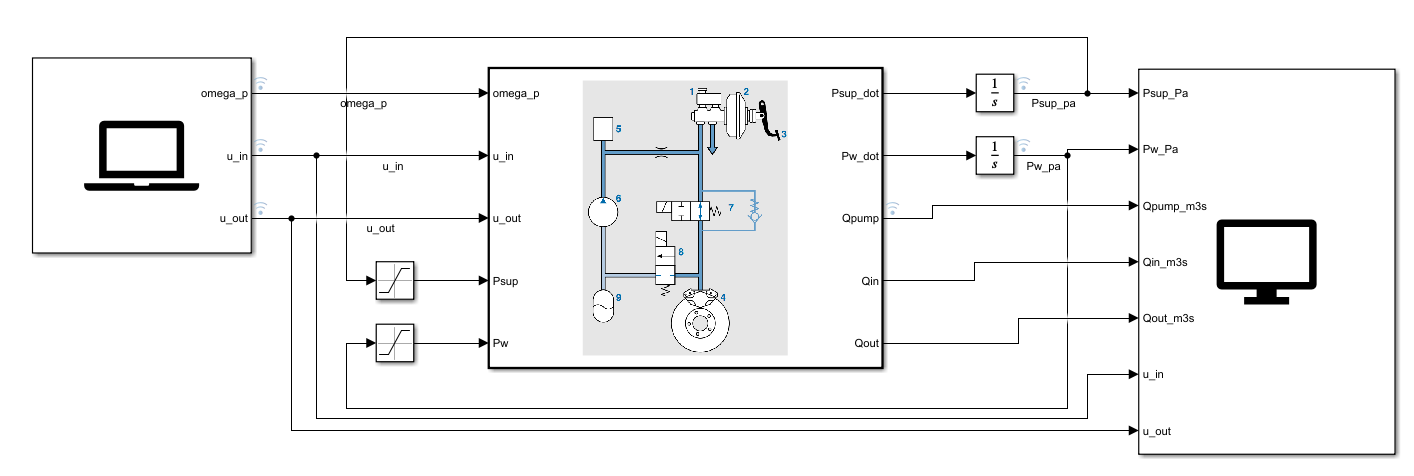
\includegraphics[width=8.2cm]{modulo_2P_malha_aberta.png}
         \caption{Circuito hidráulico: modelo concentrado em duas pressões.}
         \label{fig:modulo_2P_malha_aberta}
      \end{center}
   \end{figure}}


\subsection{Hipóteses de atuação e restrições}
O foco é o seguimento de referência de $P_w$ sob restrições físicas típicas do atuador: limites de $\omega_p$, de abertura efetiva das válvulas e faixa plausível de pressão. Além disso, por se tratar de um sistema sujeito a instrumentação limitada e incertezas de medição, considera-se a estimação de estados como parte da arquitetura de controle, uma vez que torna o controle mais preciso e robusto.

Nos ensaios, adotam-se limites de atuação coerentes com um modulador ABS/ESC em frenagem ativa, em particular $P_{sup,\max}=100\,\mathrm{bar}$ e $\omega_{p,\max}=100\,\mathrm{rad/s}$, além de comandos discretos $u_{in},u_{out}\in\{0,1\}$.

\section{Projeto do regulador digital em tempo discreto}
\label{sec:controle}
A estratégia de controle proposta combina: (i) um regulador em espaço de estados para a variável contínua $\omega_p$ e (ii) uma lógica discreta para $u_{in}$ e $u_{out}$, de modo a refletir a natureza de atuação do modulador em arquiteturas convencionais. A síntese é feita em tempo discreto para preservar coerência com implementação embarcada \cite{FranklinPowellWorkman1998,Ogata1997}.

\subsection{Linearização local e discretização}
Como a planta representada pelas Equações \eqref{eq:pressure_sup} a \eqref{eq:qout} é não linear (principalmente pela dependência em $\sqrt{\Delta P}$), adota-se uma linearização local em torno de um ponto de operação de frenagem $(x_0,u_0)$ escolhido em uma condição representativa de frenagem ativa, com $P_{sup,0}>P_{w,0}>P_{ret}$ e diferencial de pressão positivo nas válvulas. A escolha do ponto de operação foi guiada por uma condição de pressão compatível com a faixa de atuação esperada do modulador e por uma vizinhança suficientemente pequena para manter a validade local da aproximação linear. A partir disso, obtém-se um modelo linear incremental no formato:
\begin{equation}
   \delta \dot{x}(t)=A\,\delta x(t)+B\,\delta u(t),
   \qquad
   \delta y(t)=C\,\delta x(t),
   \label{eq:lin_ss}
\end{equation}
com $y(t)=P_w(t)$ como variável controlada. Para síntese digital, o modelo é discretizado com retenção de ordem zero (ZOH), resultando em $(A_d,B_d,C_d)$.

\subsection{Controlador LQI e tratamento de saturações}
Para garantir erro estacionário nulo no seguimento de patamares de referência, incorpora-se ação integral sobre o erro $e(k)=P_{\mathrm{ref}}(k)-P_w(k)$, obtendo uma formulação LQI. Os pesos do problema quadrático foram escolhidos para equilibrar rastreamento rápido e esforço moderado de controle, de modo a reduzir saturações excessivas em $\omega_p$ sem comprometer o erro em regime. O ganho do observador foi ajustado com pólos mais rápidos que a dinâmica nominal da planta, porém suficientemente amortecidos para evitar amplificação de ruído de medição, em consonância com o período de amostragem adotado. Em termos conceituais, o regulador resolve um problema de minimização quadrática em tempo discreto e gera a lei de controle:
\begin{equation}
   \omega_p(k) = \mathrm{sat}\big(\omega_{p,\min},\omega_{p,\max},\; -K_x\,\hat{x}(k)-K_i\,x_i(k)\big),
   \label{eq:lqi_control}
\end{equation}
em que $x_i$ é o estado integrador e $\hat{x}$ é o estado estimado. A saturação é explicitada para manter coerência com limites de atuação e evitar comandos inviáveis. Para reduzir risco de \textit{windup} do integrador sob saturação, emprega-se uma estratégia de anti-\textit{windup} compatível com implementação discreta \cite{FranklinPowellWorkman1998,Ogata1997}.

\subsection{Observador discreto de Luenberger}
Como o modelo possui mais estados do que medições diretas, utiliza-se um observador discreto de Luenberger para reconstruir estados necessários à lei de controle:
\begin{equation}
   \hat{x}(k+1)=A_d\hat{x}(k)+B_d u(k)+L\big(y(k)-C_d\hat{x}(k)\big),
   \label{eq:luenberger}
\end{equation}
onde $L$ é escolhido para garantir dinâmica de estimação suficientemente rápida e robusta ao ruído de medição, dentro das limitações do período de amostragem.

\subsection{Lógica discreta para válvulas}
As válvulas são comandadas por uma lógica simples baseada no erro de seguimento, com histerese para evitar comutação excessiva na presença de ruído e discretização:
\begin{itemize}
   \item se $e(k)>\varepsilon$: prioriza-se pressurização ($u_{in}=1$, $u_{out}=0$);
   \item se $e(k)<-\varepsilon$: prioriza-se alívio ($u_{in}=0$, $u_{out}=1$);
   \item se $|e(k)|\le \varepsilon$: aplica-se retenção (\textit{hold}) ($u_{in}=0$, $u_{out}=0$).
\end{itemize}
Esse arranjo busca representar, de modo controlável, os três modos clássicos do canal hidráulico (pressurizar, reter, aliviar) \cite{Konrad2014}, sem assumir válvulas plenamente proporcionais.

\section{Cenários de simulação e critérios de avaliação}
\label{sec:simulacao}
A avaliação em simulação considera ensaios em malha aberta e em malha fechada. A malha aberta tem caráter de verificação de plausibilidade do modelo e exercita os três modos típicos do canal hidráulico (pressurizar, reter e aliviar). A malha fechada permite discutir seguimento de referência e esforço de atuação sob saturações. Para facilitar a leitura, as pressões são apresentadas em $\mathrm{bar}$ nas figuras.

Para discutir sensibilidade a ruído de medição, considera-se o caso em que a pressão medida e disponibilizada ao observador é modelada por:
\begin{equation}
   y(k)=P_w(k)+n(k),
   \label{eq:meas_noise_model}
\end{equation}
onde $n(k)$ é um ruído branco de média zero. No modelo, $P_w$ permanece como a pressão ``verdadeira'' do canal de roda, enquanto $y(k)$ é o sinal usado pelo observador \eqref{eq:luenberger} e, por consequência, pela lei de controle.

A discussão é apoiada em métricas usuais de desempenho, tais como erro RMS, sobressinal, tempos característicos (subida/acomodação), erro estacionário e esforços máximos de controle. Além disso, a robustez é discutida por meio de variação paramétrica em torno do caso nominal, observando-se a degradação de desempenho sob variações de parâmetros físicos (por exemplo, volumes equivalentes, módulo volumétrico efetivo e coeficientes associados à bomba e às válvulas), abordagem alinhada ao uso de simulação como etapa de verificação em sistemas de controle embarcados \cite{KapinskiJamesDeshmukh2016}.

A Figura~\ref{fig:modulo_2P_malha_fechada} apresenta o modelo Simulink utilizado para os ensaios, com os blocos de planta, controlador e lógica de válvulas destacados. O modelo inclui a possibilidade de adicionar ruído de medição e variação paramétrica para análise de sensibilidade.

\IfFileExists{modulo_2P_malha_fechada.png}{%
   \begin{figure}
      \begin{center}
         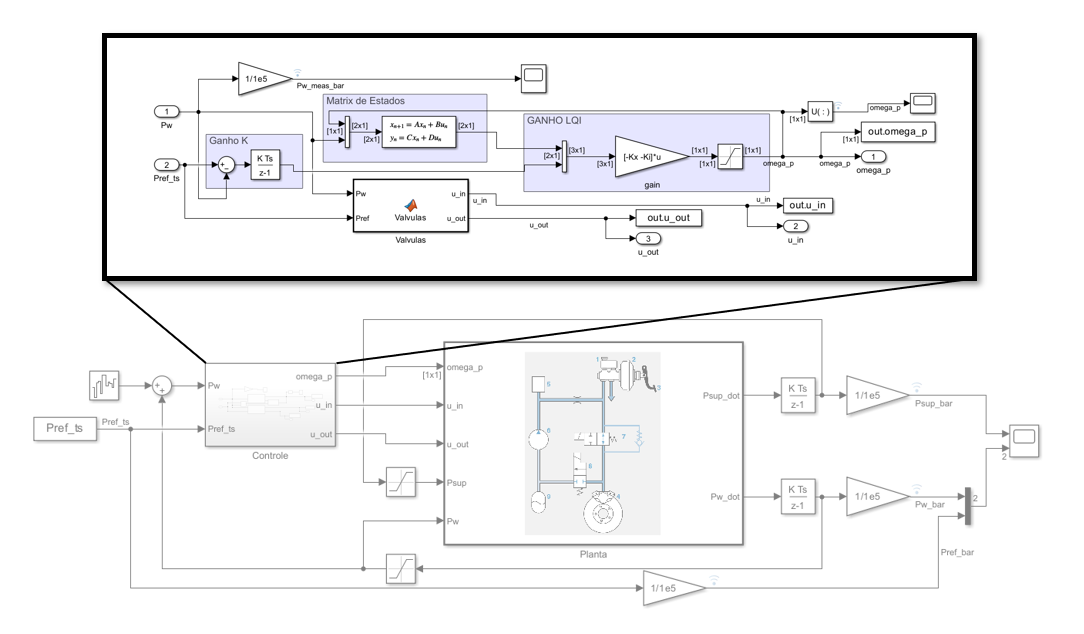
\includegraphics[width=8.2cm]{modulo_2P_malha_fechada.png}
         \caption{Modelo Simulink dos ensaios (planta, controlador e lógica de válvulas).}
         \label{fig:modulo_2P_malha_fechada}
      \end{center}
   \end{figure}}



\section{Resultados e discussão}
\label{sec:resultados}
Esta seção organiza os resultados em dois blocos: (i) verificação em malha aberta, para checar coerência causal e ordem de grandeza da planta não linear; e (ii) ensaios em malha fechada, para discutir seguimento de referência de $P_w$, saturações e a sensibilidade do regulador à instrumentação (ruído de medição).

Por consistência com as figuras, as pressões são apresentadas em $\mathrm{bar}$ e interpretadas em relação ao retorno $P_{ret}$. Assim, quando conveniente, utiliza-se a conversão:
\begin{equation}
   P_g = \frac{P-P_{ret}}{10^5},
   \label{eq:pg_def}
\end{equation}
onde $P$ e $P_{ret}$ estão em Pa.

Em malha aberta (Figura~\ref{fig:artigo_ensaio_malha_aberta_integrado_real}), observa-se coerência causal entre comandos e variação de pressão: pressurização eleva $P_{sup}$ e $P_w$, retenção estabiliza o canal e alívio reduz $P_w$ via válvula de saída. Essa verificação minimiza o risco de atribuir ao regulador efeitos decorrentes de inconsistências de modelagem \cite{HouhuaJing2022,ZengYangHuang2023}.

\begin{figure}
   \begin{center}
      \figpdforpng{artigo_ensaio_malha_aberta_integrado_real}
      \caption{Malha aberta: pressurização, retenção e alívio.}
      \label{fig:artigo_ensaio_malha_aberta_integrado_real}
   \end{center}
\end{figure}

Em malha fechada (Figura~\ref{fig:simulacao_comandos_e_pressao}), a arquitetura LQI+observador rastreia referências em patamares no modelo não linear com comandos compatíveis com as restrições impostas a $\omega_p$, $u_{in}$ e $u_{out}$. Para condensar os destaques do cenário nominal, a Tabela~\ref{tab:resumo_desempenho} resume os principais compromissos observados no ensaio em malha fechada, enquanto a leitura conjunta de pressão e atuação orienta a discussão de seguimento, saturações e efeitos de não linearidade (dependência das vazões em $\Delta P$), incluindo possíveis assimetrias entre pressurização e alívio \cite{Lv2014,ChenLv2017}.

\begin{table}[t]
   \centering
   \caption{Resumo dos resultados em malha fechada.}
   \label{tab:resumo_desempenho}
   \begin{tabular}{p{3.6cm}p{4.1cm}}
      \toprule
      Cenário                   & Destaque principal                                                                                                                \\
      \midrule
      Seguimento por degraus    & O controlador acompanha os patamares de referência com erro reduzido em regime e transitórios dominados pela dinâmica hidráulica. \\
      Saturação e esforço       & O comando de $\omega_p$ atinge limites de atuação em transições agressivas, mas sem perda de coerência do comportamento.          \\
      Ruído de medição          & O observador preserva o rastreamento, com aumento moderado de ripple e esforço de controle.                                       \\
      Sensibilidade paramétrica & O desempenho permanece aceitável para variações moderadas de $\beta$, $V_w$ e $A_{in,\max}$.                                      \\
      \bottomrule
   \end{tabular}
\end{table}

\begin{figure}
   \begin{center}
      \figpdforpng{simulacao_comandos_e_pressao}
      \caption{Malha fechada: pressão e comandos de atuação.}
      \label{fig:simulacao_comandos_e_pressao}
   \end{center}
\end{figure}

\IfFileExists{artigo_item01_metricas_tracking.png}{%
   \begin{figure}
      \begin{center}
         
\includegraphics[width=8.2cm]{artigo_item01_metricas_tracking.png}
         \caption{Seguimento por degraus: resposta e erro.}
         \label{fig:artigo_item01_metricas_tracking}
      \end{center}
   \end{figure}

   A Figura~\ref{fig:artigo_item01_metricas_tracking} apresenta o seguimento de referência por múltiplos degraus. Observa-se que os maiores desvios concentram-se nos instantes de transição, enquanto em regime o erro se mantém reduzido, o que é consistente com a atuação do LQI com observador.

   \begin{figure}
      \begin{center}
         
\includegraphics[width=8.2cm]{artigo_item01_metricas_desempenho.png}
         \caption{Métricas globais e por degrau do seguimento.}
         \label{fig:artigo_item01_metricas_desempenho}
      \end{center}
   \end{figure}

   A Figura~\ref{fig:artigo_item01_metricas_desempenho} resume métricas por degrau (sobressinal, tempos característicos, erro estacionário e erro RMS). Em conjunto, as Figuras~\ref{fig:artigo_item01_metricas_tracking}--\ref{fig:artigo_item01_metricas_desempenho} sustentam uma leitura objetiva do compromisso entre rapidez e precisão ao longo da faixa de patamares ensaiada.
}{ }

\IfFileExists{artigo_item02_dpdt_saturacao.png}{%
   \begin{figure}
      \begin{center}
         
\includegraphics[width=8.2cm]{artigo_item02_dpdt_saturacao.png}
         \caption{Taxas $\mathrm{d}P/\mathrm{d}t$ e saturação do comando.}
         \label{fig:artigo_item02_dpdt_saturacao}
      \end{center}
   \end{figure}

   A Figura~\ref{fig:artigo_item02_dpdt_saturacao} explicita limites dinâmicos do atuador ao relacionar taxas $\mathrm{d}P/\mathrm{d}t$ e saturação de comando. Observa-se que, mesmo próximo ao limite superior de atuação, os picos de $\left|\mathrm{d}P_w/\mathrm{d}t\right|$ permanecem confinados, indicando um teto imposto pela dinâmica hidráulica (dependência em $\Delta P$ e $\beta/V$), e não apenas pelo esforço do regulador.
}{ }

\IfFileExists{artigo_item03_assimetria_subida_descida.png}{%
   \begin{figure}
      \begin{center}
         
\includegraphics[width=8.2cm]{artigo_item03_assimetria_subida_descida.png}
         \caption{Pressurização vs. alívio: resposta e comandos.}
         \label{fig:artigo_item03_assimetria_subida_descida}
      \end{center}
   \end{figure}

   A Figura~\ref{fig:artigo_item03_assimetria_subida_descida} evidencia assimetria entre pressurização e alívio, comportamento esperado quando os caminhos de fluxo e as condições de $\Delta P$ diferem nos dois sentidos. Essa leitura é importante porque o desempenho pode ser limitado pela física do circuito (e não pelo regulador), e deve ser reportado de forma objetiva antes de extrapolar conclusões sobre o controlador \cite{Lv2014,ChenLv2017}.
}{ }

\IfFileExists{artigo_item04_ripple_fft.png}{%
   \begin{figure}
      \begin{center}
         
\includegraphics[width=8.2cm]{artigo_item04_ripple_fft.png}
         \caption{Ondulação em regime: erro no tempo e espectro.}
         \label{fig:artigo_item04_ripple_fft}
      \end{center}
   \end{figure}

   Para além do erro médio, a ondulação em regime (Figura~\ref{fig:artigo_item04_ripple_fft}) caracteriza flutuações associadas à lógica discreta de válvulas e ao período de amostragem. A inspeção temporal e espectral do erro em patamar ajuda a distinguir erro de seguimento lento de oscilações de alta frequência que podem elevar comutação e esforço de atuação.
}{ }

\IfFileExists{artigo_item05_validacao_linearizacao.png}{%
   \begin{figure}
      \begin{center}
         \includegraphics[width=8.2cm]{artigo_item05_validacao_linearizacao.png}
         \caption{Planta não linear vs. modelo linearizado (janela de operação).}
         \label{fig:artigo_item05_validacao_linearizacao}
      \end{center}
   \end{figure}

   Como a síntese do LQI depende da linearização local, a Figura~\ref{fig:artigo_item05_validacao_linearizacao} é usada como checagem de consistência em pequena vizinhança do ponto de operação. Diferenças residuais entre as curvas indicam o grau de não linearidade efetivamente excitado e ajudam a delimitar a faixa de validade do projeto linear, sem sugerir equivalência global entre modelos.
}{ }

\IfFileExists{artigo_item06_sensibilidade_parametrica.png}{%
   \begin{figure}
      \begin{center}
         
\includegraphics[width=8.2cm]{artigo_item06_sensibilidade_parametrica.png}
         \caption{Sensibilidade paramétrica: métricas de erro e esforço.}
         \label{fig:artigo_item06_sensibilidade_parametrica}
      \end{center}
   \end{figure}

   A Figura~\ref{fig:artigo_item06_sensibilidade_parametrica} discute robustez por variação paramétrica em torno do caso nominal, focalizando parâmetros com interpretação física direta ($\beta$, $V_w$ e $A_{in,\max}$). Na faixa avaliada, as métricas agregadas de erro RMS e esforço RMS apresentam variação limitada, sugerindo baixa sensibilidade do seguimento a perturbações moderadas nesses parâmetros.
}{ }

\IfFileExists{artigo_item07_atrasos_tempos.png}{%
   \begin{figure}
      \begin{center}
         
\includegraphics[width=8.2cm]{artigo_item07_atrasos_tempos.png}
         \caption{Atraso e tempo de subida por degrau.}
         \label{fig:artigo_item07_atrasos_tempos}
      \end{center}
   \end{figure}

   A Figura~\ref{fig:artigo_item07_atrasos_tempos} organiza atrasos e tempos característicos por degrau, fornecendo uma visão compacta de ``largura de banda'' observada no canal de pressão. Esses indicadores são úteis para diferenciar limitações do atuador hidráulico de efeitos de discretização e de estimação em tempo discreto.
}{ }

\IfFileExists{artigo_item08_mapa_comando_pressao.png}{%
   \begin{figure}
      \begin{center}
         
\includegraphics[width=8.2cm]{artigo_item08_mapa_comando_pressao.png}
         \caption{Mapas comando--efeito: comando vs. $\mathrm{d}P/\mathrm{d}t$.}
         \label{fig:artigo_item08_mapa_comando_pressao}
      \end{center}
   \end{figure}

   A Figura~\ref{fig:artigo_item08_mapa_comando_pressao} relaciona comandos ($\omega_p$, $u_{in}$ e $u_{out}$) e taxas $\mathrm{d}P/\mathrm{d}t$, evidenciando dependência do ganho hidráulico em relação a $\Delta P$ e ao regime de operação. Esses mapas reforçam a natureza não linear do canal de pressão e justificam a avaliação do controle diretamente no modelo não linear \cite{ChenLv2017,Lv2014}.
}{ }

\IfFileExists{artigo_item09_tradeoff_erro_esforco.png}{%
   \begin{figure}
      \begin{center}
         
\includegraphics[width=8.2cm]{artigo_item09_tradeoff_erro_esforco.png}
         \caption{Trade-off erro--esforço (variação de $R$).}
         \label{fig:artigo_item09_tradeoff_erro_esforco}
      \end{center}
   \end{figure}

   Para evitar conclusões dependentes de um único ajuste, a Figura~\ref{fig:artigo_item09_tradeoff_erro_esforco} explicita o compromisso entre erro e esforço de atuação associado a escolhas de ponderação do LQI. Essa apresentação é particularmente relevante em moduladores eletro-hidráulicos, nos quais reduzir erro pode elevar saturações, comutação e desgaste.
}{ }

\IfFileExists{artigo_item10_robustez_ruido.png}{%
   \begin{figure}
      \begin{center}
         
\includegraphics[width=8.2cm]{artigo_item10_robustez_ruido.png}
         \caption{Ruído de medição: métricas globais vs. nível de ruído.}
         \label{fig:artigo_item10_robustez_ruido}
      \end{center}
   \end{figure}

   A Figura~\ref{fig:artigo_item10_robustez_ruido} resume o efeito do ruído de medição da pressão sobre as métricas globais de erro e esforço, complementando a Figura~\ref{fig:artigo_simulacao_ruido_medicao} com uma leitura agregada do impacto do ruído. À medida que o desvio padrão do ruído aumenta, observa-se um crescimento gradual do erro RMS e do esforço RMS do atuador, bem como um aumento na atividade de controle associada às correções sucessivas. No entanto, essa degradação é moderada na faixa de ruídos analisada (até 1~bar), sem indicar perda abrupta de desempenho.

   Esses resultados sugerem que o arranjo controlador--observador é capaz de tolerar níveis de ruído compatíveis com sensores reais de pressão, ainda que à custa de um aumento previsível na comutação e no desgaste dos atuadores. Do ponto de vista de projeto, isso indica que a escolha de sensores com qualidade razoável é suficiente para preservar o comportamento desejado, sem necessidade de requisitos excessivamente restritivos quanto a ruído.
}{ }

\IfFileExists{artigo_item11_transicoes_referencia.png}{%
   \begin{figure}
      \begin{center}
         
\includegraphics[width=8.2cm]{artigo_item11_transicoes_referencia.png}
         \caption{Transições de referência por patamares.}
         \label{fig:artigo_item11_transicoes_referencia}
      \end{center}
   \end{figure}

   Embora o foco seja o regulador de baixa camada, as transições de patamar (Figura~\ref{fig:artigo_item11_transicoes_referencia}) representam mudanças de demanda compatíveis com integração a funções ADAS longitudinais, nas quais $P_{ref}$ é imposto por um controlador superior. A avaliação por segmentos permite discutir coerência do seguimento sob mudanças sucessivas de demanda, sem assumir um modelo completo de veículo.
}{ }

\IfFileExists{artigo_item12_plausibilidade_resumo.png}{%
   \begin{figure}
      \begin{center}
         
\includegraphics[width=8.2cm]{artigo_item12_plausibilidade_resumo.png}
         \caption{Resumo de ordens de grandeza (pressões, picos e tempos).}
         \label{fig:artigo_item12_plausibilidade_resumo}
      \end{center}
   \end{figure}

   A Figura~\ref{fig:artigo_item12_plausibilidade_resumo} consolida, em um único painel, a curva base de referência e as principais ordens de grandeza extraídas das simulações. As faixas de pressão observadas em $P_w$ e $P_{sup}$, os picos de $\left|\mathrm{d}P/\mathrm{d}t\right|$, os limites de $\omega_p$ e os tempos típicos de subida e acomodação são compatíveis com o que se espera para moduladores hidráulicos empregados em sistemas de freio automotivos.

   A consistência dessas ordens de grandeza com tendências reportadas na literatura e com especificações usuais de sistemas ABS/ESC reforça a plausibilidade física do modelo utilizado \cite{HouhuaJing2022,ZengYangHuang2023,Lv2014,ChenLv2017}. Assim, além de servir como ferramenta de projeto e avaliação de controle, o modelo concentrado adotado mostra-se aderente ao comportamento qualitativo e quantitativo de moduladores reais, o que é um requisito importante para a relevância prática dos resultados apresentados.
}{ }

\IfFileExists{artigo_extra_discretizacao.png}{%
   \begin{figure}
      \begin{center}
         
\includegraphics[width=8.2cm]{artigo_extra_discretizacao.png}
         \caption{Sensibilidade ao período de amostragem $T_s$.}
         \label{fig:artigo_extra_discretizacao}
      \end{center}
   \end{figure}

   Em aplicações embarcadas, a escolha de $T_s$ influencia simultaneamente desempenho, esforço e robustez do observador. Assim, a Figura~\ref{fig:artigo_extra_discretizacao} é usada para discutir a sensibilidade do desempenho à discretização e separar limitações do atuador hidráulico de artefatos numéricos associados ao laço digital.
}{ }

\IfFileExists{artigo_simulacao_ruido_medicao.png}{%
   \begin{figure}
      \begin{center}
         \figpdforpng{artigo_simulacao_ruido_medicao}         \caption{Malha fechada com ruído na medição de $P_w$.}
         \label{fig:artigo_simulacao_ruido_medicao}      \end{center}
   \end{figure}

   A Figura~\ref{fig:artigo_simulacao_ruido_medicao} ilustra, no tempo, o impacto do ruído de medição na trajetória de seguimento. Observa-se aumento de flutuações em torno dos patamares (\textit{ripple}), enquanto a capacidade de rastreamento é preservada no cenário avaliado, em consonância com a síntese agregada apresentada na Figura~\ref{fig:artigo_item10_robustez_ruido}.
}{}

Em síntese, os resultados desta seção estabelecem (i) coerência causal e ordem de grandeza do modelo não linear em malha aberta e (ii) viabilidade de seguimento de referência em malha fechada sob restrições de atuação e lógica discreta. Esses achados delimitam o que o modelo e o regulador demonstram no escopo de simulação e motivam, como passos seguintes, a consolidação de métricas sumarizadas e a exploração sistemática de sensibilidade paramétrica quando o objetivo for comparar configurações e hipóteses de modelagem.

\section{Conclusões}
\label{sec:conclusoes}
Este artigo apresentou um fluxo metodológico para projeto e avaliação, em simulação, de um regulador digital de pressão hidráulica por roda usando o módulo ABS/ESC como atuador em frenagem ativa. A combinação de modelo não linear concentrado, linearização local, síntese LQI em tempo discreto, observador de Luenberger e lógica discreta de válvulas fornece uma arquitetura compatível com restrições de atuação e com requisitos típicos de integração a funções ADAS longitudinais \cite{Lentin2022,Konrad2014}.

Os resultados devem ser interpretados dentro do escopo proposto: evidência em ambiente MATLAB/Simulink, voltada à coerência do controle e à compatibilidade com restrições de atuação e instrumentação. As simulações em malha aberta e em malha fechada organizam um conjunto mínimo de evidências para sustentar a modelagem adotada e a pertinência de combinar regulador em tempo discreto, observador e lógica de válvulas no contexto de frenagem ativa.

A seção de resultados inclui um conjunto de análises diretamente extraídas das curvas simuladas: métricas por degrau, envelopes de $\mathrm{d}P/\mathrm{d}t$ e saturações, assimetria entre pressurização e alívio, avaliação de ondulação em regime, checagem local de consistência entre modelo linearizado e planta não linear, varreduras paramétricas focadas e estudo do compromisso erro--esforço. Além disso, inclui-se uma avaliação de sensibilidade ao período de amostragem para discutir robustez da implementação discreta.

Como limitações, o estudo não pretende representar um veículo completo (dinâmica longitudinal/pneu) nem substituir validação experimental do atuador; além disso, a síntese é baseada em linearização local e a atuação de válvulas é representada por lógica binária com histerese. Como continuidade natural, destacam-se a implementação embarcada do regulador em microcontrolador automotivo, a verificação de temporização do laço de controle, o tratamento de efeitos de quantização/ruído e a validação em bancada/HIL com instrumentação mínima de pressão, de modo a consolidar a transferência do \textit{model-in-the-loop} para o ambiente físico \cite{KapinskiJamesDeshmukh2016}.

\bibliography{ifacconf}             % bib file to produce the bibliography
% with bibtex (preferred)

%\begin{thebibliography}{xx}  % you can also add the bibliography by hand

%\bibitem[Able(1956)]{Abl:56}
%B.C. Able.
%\newblock Nucleic acid content of microscope.
%\newblock \emph{Nature}, 135:\penalty0 7--9, 1956.

%\bibitem[Able et~al.(1954)Able, Tagg, and Rush]{AbTaRu:54}
%B.C. Able, R.A. Tagg, and M.~Rush.
%\newblock Enzyme-catalyzed cellular transanimations.
%\newblock In A.F. Round, editor, \emph{Advances in Enzymology}, volume~2, pages
%  125--247. Academic Press, New York, 3rd edition, 1954.

%\bibitem[Keohane(1958)]{Keo:58}
%R.~Keohane.
%\newblock \emph{Power and Interdependence: World Politics in Transitions}.
%\newblock Little, Brown \& Co., Boston, 1958.

%\bibitem[Powers(1985)]{Pow:85}
%T.~Powers.
%\newblock Is there a way out?
%\newblock \emph{Harpers}, pages 35--47, June 1985.

%\bibitem[Soukhanov(1992)]{Heritage:92}
%A.~H. Soukhanov, editor.
%\newblock \emph{{The American Heritage. Dictionary of the American Language}}.
%\newblock Houghton Mifflin Company, 1992.

%\end{thebibliography}
\end{document}

